%! Author = paolo
%! Date = 03/02/2023

% Preamble
\documentclass[11pt]{article}

% Packages
\usepackage{amsmath}
\usepackage[margin = .3in]{geometry}
\usepackage{amssymb}
\usepackage{graphicx}
\usepackage{caption}
\usepackage{graphics}
\usepackage{multicol}
\usepackage{bm}

\renewcommand*\contentsname{Indice}

\begin{document}
    \tableofcontents
    \newpage

    \section{Formule sparse}

    Coefficiente di correlazione lineare: $ r = \frac{\sigma_{xy}}{\sigma_x \sigma_y} =
    \frac{\sum (x_i - \bar{x})(y_i - \bar{y})}{\sqrt {\sum (x_i  - \bar{x})^2 \sum (y_i - \bar{y})^2}} \; \; r \in [-1 ; 1] $ \hfill \\[.7\baselineskip]
    Covarianza: $ \sigma_{xy} = \frac{1}{N} \sum (x_i - \overline{x})(y_i - \overline{y}) $ \hfill \\[.7\baselineskip]
    Deviazione std (s.q.m): $s_x = \sqrt {\frac{1}{N-1} \sum d_i^2} = \sqrt {\frac{1}{N-1} \sum (x_i - \overline{x})^2}$
    (incertezza sulla singola misura) \hfill \\[.7\baselineskip]
    Deviazione std della media: $s_{\overline{x}} = \sqrt {\frac{1}{N(N-1)} \sum (x_i - \overline{x})^2} = \frac{s_x}{\sqrt {N}} $ \hfill \\[.7\baselineskip]
    Densità di frequenza: $\varPhi_{k} = \frac{f_{k}}{\Delta x}$. $\Delta x$: ampiezza bin, $f_k = \frac{n_k}{N}$, k: indice del bin. \hfill \\[.7\baselineskip]
    Media aritmetica: $\frac{\sum x_i}{N}$ oppure $\frac{\sum n_kx_k}{N}$ \hfill \\[.7\baselineskip]
    Scarto quadratico medio (dev std): $s_x = \sqrt {\frac{1}{N-1} \sum d_i^2} = \sqrt {\frac{1}{N-1} \sum (x_i - \overline{x})^2}$ \hfill \\[.7\baselineskip]
    Scarto medio: $\frac{1}{N} \sum |d_i|$. $d_i = x_i - \overline{x}$ \hfill \\[.7\baselineskip]
    Varianza: $s_x^2 = \frac{N}{N-1}(\overline{x^2} - \overline{x}^2) $


    \section{Calcolo combinatorio}

    \paragraph{Disposizioni}numero di modi diversi di disporre k oggetti, presi da un insieme di n oggetti (n nPr k).
    \[ \frac{n!}{(n - k)!} \]

    \paragraph{Combinazioni}numero di sottogruppi da k elementi possibili in un gruppo di n elementi (n nCr k).
    \[ \frac{n!}{(n - k)! \, k!} = \binom{n}{k} \]


    \section{Propagazione degli errori}

    \subsection{Propagazione lineare}
    $a = f(x) \Rightarrow \Delta a = \bigg|\frac{\partial f}{\partial x}\bigg|_{
        \fontsize{5}{5}\selectfont
        \begin{aligned}
            x &=  \overline{x} \\
            y &=  \overline{y}
        \end{aligned}} \cdot \Delta x $

    \subsection{Propagazione in quadratura}
    data $ q(x, y), \sigma_x $ e $ \sigma_y $ allora $ \overline{q} = q(\overline{x}, \overline{y}) $ e
    $ \sigma_q = \sqrt{\left( \frac{\partial q}{\partial x} \right)^2 (\sigma_x)^2 +
    \left( \frac{\partial q}{\partial y} \right)^2 (\sigma_y)^2 +
    2 \, \frac{\partial q}{\partial x} \frac{\partial q}{\partial y} \sigma_{xy} } $ \\
    se le variabili non sono correlate ($ \sigma_{xy} = 0 $) allora la formula si riduce a:
    $ \sigma_q = \sqrt{\left( \frac{\partial q}{\partial x} \right)^2 (\sigma_x)^2 +
    \left( \frac{\partial q}{\partial y} \right)^2 (\sigma_y)^2 } $

    \subsection{Media pesata}
    Date due misure $ (x_1 \pm \sigma_1) $ e $ (x_2 \pm \sigma_2) $ compatibili tra loro, è possibile ricavare la miglior
    stima del valore $ x_p = \frac{w_1 \cdot x_1 + w_2 \cdot x_2}{w_1 + w_2} $, dove $w_i = \frac{1}{\sigma_i^2} $ e
    la dev std $ \sigma_p = \frac{1}{\sqrt{w_1 + w_2}} $


    \section{Rigetto dati}

    \subsection{Criterio di Chauvenet}
    Data la misura sospetta $x_s$, se $ P\left(|z| > \frac{x_s - \mu}{\sigma} \right) \cdot N < 0.5 $ allora la misura
    $x_s$ può essere rigettata.\\
    Successivamente bisogna ricalcolare media e deviazione std (quest'ultima è difficile).

    \subsection{Caso campioni ridotti}
    Se $ P \left( |t| > \frac{x_s - \overline{x}}{\sigma_x} \right) \cdot N < 0.5 $ allora può essere rigettata. \\
    Usa $ \sigma_x $ non $\sigma_{\overline{x}}$


    \section{Valutazione delle ipotesi}

    \subsection{Test delle ipotesi}
    Dato un valore accettato $v_{acc}$ e una serie di $N$ misure con media $\overline{x}$ e dev std $ \sigma_x $,
    si calcola $ \sigma_{\overline{x}} = \frac{\sigma_x}{\sqrt{N}} $ poi si calcola
    $ z = \frac{\overline{x} - v_{acc}}{\sigma_{\overline{x}}} $ e, se $N$ è grande si usa $G(z)$ altrimenti $S_\nu(z)$. \hfill \break
    Bisogna prendere entrambe le code, quindi moltiplicare per 2.
    Se il valore trovato è minore di 0.05 allora c'è discrepanza, se è minore di 0.01 questa è critica. \hfill \break
    Se si deve determinare la compatibilità di due misure, senza la presenza di un valore accettato si calcola:
    \begin{itemize}
        \item se le popolazioni sono ridotte:
        $ t = \frac{\overline{x_1} - \overline{x_2}}{\sqrt{\left( \frac{n_1 - 1}{n_1 + n_2 - 2}\sigma_1^2 +
        \frac{n_2 - 1}{n_1 + n_2 - 2}\sigma_2^2 \right) \left( \frac{1}{n_1} + \frac{1}{n_2} \right)}} $ con $ \nu = n_1 + n_2 - 2 $
        \item se le popolazioni sono numerose:
        $ z = \frac{|\overline{x_1} - \overline{x_2}|}{\sqrt{\frac{\sigma_1^2}{n_1} + \frac{\sigma_2^2}{n_2}}} $
        $\left( \frac{\sigma_1^2}{n_1} = \sigma_{\overline{x}}^2 \right) $
    \end{itemize}

    \subsection{Test correlazione lineare}

    Per verificare l'ipotesi di correlazione lineare calcolo il coefficiente di correlazione lineare: \\[.3\baselineskip]
    $ r_0 = \frac{\sigma_{xy}}{\sigma_x \sigma_y} =
    \frac{\sum (x_i - \bar{x})(y_i - \bar{y})}{\sqrt {\sum (x_i  - \bar{x})^2 \sum (y_i - \bar{y})^2}} \; \; r \in [-1 ; 1] $
    e controllo sulla tabella la probabilità $ P_N(|r| > r_0) $ se $ P < 0.05 $ l'ipotesi di correlazione lineare è buona,
    se $P < 0.01 $ è ottima.

    \subsection{Test del $\chi^2$}
    \subsubsection{Verifica distribuzione di probabilità/PDF}
    Dato un set di $N$ risultati divisi in $n$ bin del tipo $[a_i; b_i]$ o $x_i$ e una pdf $ \Phi(x; \alpha; \dots) $ o
    una ditribuzione di probabilità $P(k; \alpha; \dots)$ dove $ \alpha; \, \dots $ sono gli altri parametri;
    chiamo $O_i$ il numero di eventi in un bin, $E_i$ il numero di eventi previsti da $\Phi$ o $P$ e $\sigma_i$ l'errore
    su $O_i$
    \begin{itemize}
        \item $O_i$ lo prendo dal set di risultati
        \item se ho una pdf $E_i = N \int_{a_i}^{b_i} \Phi(x) \, dx = N \, p_i $
        \item se ho una distr. di prob. $E_i = N P(x_i) = N \, p_i $
        \item se $p_i \ll 1 $ (molti bin) allora $\sigma_i^2 = Np_i = E_i $ (variabile poissoniana)
        \item altrimenti $\sigma_i^2 = N p_i (1 - p_i) $ (variabile binomiale)
    \end{itemize}
    \[ \chi^2 = \sum_{0}^{n} \frac{\left( O_i - E_i \right)^2}{\sigma_i^2} \]
    Ora bisogna determinare i gradi di libertà $\nu$;
    in genere sono $n -1$ ma per ogni parametro della pdf/dist. stimato a partire dai risultati se ne
    perde un'altro. \\
    Se l'ipotesi è corretta $ \chi^2 \approx \nu $, se no $ \chi^2 \gg \nu $, $ \chi^2 \gg \nu $ può voler dire che
    l'errore è stato sovrastimato. \\
    Per praticità introduciamo il $\chi^2$ ridotto: $ \tilde{\chi}^2 = \frac{\chi^2}{\nu} \approx 1 $ se l'ipotesi è corretta. \\
    Se $P_\nu (\chi^2 > \chi_0^2) < 0.05$ c'è discrepanza, se $< 0.01$ questa è netta.
    \paragraph{Attenzione}
    \begin{itemize}
        \item il numero di misure in ogni bin dev'essere $\geq 4-5$
        \item bisogna avere abbastanza bin affinché $\nu > 0$
    \end{itemize}
    
    \subsubsection{Verifica relazione funzionale}
    Dato un insieme di $N$ coppie $(x_i, y_i \pm \sigma_i)$ e una funzione $f(x; \alpha; \dots )$
    \[ \chi^2 = \sum_{0}^{N} \left( \frac{y_i - g(x_i)}{\sigma_i} \right)^2 \]
    I gradi di libertà sono: $\nu = N - $ il numero di parametri $\alpha, \dots$ dedotti dai dati.
    Ora calcolo il $\tilde{\chi}^2 = \frac{\chi^2}{\nu} $ e la trattazione è uguale a quella per il caso precedente.

    \section{Regressione lineare}
    \subsection{Caso base}
    Dato un insieme di misure: $x_i (y_i \pm \sigma_{yi}) $, nell'ipotesi che: \\
    - $y_i$ siano estratti da popolazioni gaussiane \\
    - $\sigma_yi = \sigma_yj \; \forall \: i,j $ \\
    Le migliori stime di $m$ e $q$ e delle loro incertezze sono:
    \begin{gather*}
        m = \frac{N \sum x_i y_i - \sum x_i \sum y_i}{\Delta}\qquad
        q = \frac{\sum x_i^2 \sum y_i  - \sum x_i \sum x_i y_i}{\Delta} \qquad
        \Delta = N \sum x_i^2 - \left( \sum x_i \right)^2 \\
        \sigma_m = \sigma_y \sqrt {\frac{N}{\Delta}} \qquad
        \sigma_q = \sigma_y \sqrt {\frac{\sum x_i^2}{\Delta}}
    \end{gather*}
    Se non ho $\sigma_y$ posso stimarla (e usarla per calcolare $\sigma_m$ e $\sigma_q$) come
    $ \hat{\sigma_y} = \sqrt {\frac{1}{N - 2} \sum \left( y_i - mx_i - q \right)^2} $

    \subsubsection{Intercetta a 0}
    \begin{gather*}
        m = \frac{\sum x_i y_i}{\sum x_i^2} \qquad \sigma_m = \frac{\sigma_y}{\sqrt{\sum x_i^2}}
    \end{gather*}

    \subsection{Incertezze sulle y variabili}
    In questo caso peso i vari punti in base all'errore: peso $w_i = \frac{1}{\sigma_i^2}$ \\
    E ottengo:
    \begin{gather*}
        m = \frac{\sum w_i \sum w_i x_i y_i - \sum w_i x_i \sum w_i y_i}{\Delta}\quad
        q = \frac{\sum w_i x_i^2 \sum w_i y_i  - \sum w_i x_i \sum w_i x_i y_i}{\Delta} \quad
        \Delta = \sum w_i \sum w_i x_i^2 - \left( \sum w_i x_i \right)^2
    \end{gather*}
    (Il cuffia rimanda al par 10.3 del Fornasini per $\sigma_m$ e $\sigma_q$)

    \subsection{Errori in x non trascurabili}
    Calcolo m ignorando gli errori su x. Poi calcolo un $\sigma_y$ equivalente: $\sigma_{y \, eq} = m \sigma_x$. \\
    Infine $ \sigma_{y \, tot} = \sqrt{\sigma_y^2 + \sigma_{y \, eq}^2} $ e mi riconduco al caso delle sole incertezze
    sulle y variabili

    \section{PDF}

    \subsection{caratteristiche PDF}
    Normalizzazione: $ 1 = \int \Phi(x) dx $ \\[.3\baselineskip]
    Media: $\overline{x} = \int x \Phi(x) dx $ \\[.3\baselineskip]
    Varianza: $ s_x^2 = \int (x - \overline{x})^2 \Phi(x) dx $

    \subsection{Gaussiana}
    \[ \Phi (x) = \frac{1}{\sigma \sqrt{2 \pi}} \, e^{- \frac{(x - \mu)^2}{2 \sigma^2}} \] \hfill
    \begin{center}
        \begin{minipage}{.75\textwidth}
            $\overline{x} = \mu $ \hfill $ s_x^2 = \sigma^2 $ \hfill $ z = \frac{x - \mu}{\sigma} $ \hfill
            $ \hat{\mu} = \overline{x} $ \hfill $\hat{\sigma}^2 = s_x^2 $ \hfill FWHM $ = 2 \sigma \sqrt{\ln 4} $ \hfill
        \end{minipage}
    \end{center}
    La combinazione $ q = c_1 x + c_2 y $ di due variabili gaussiane è a sua volta gaussiana; \\
    media: $ \mu = c_1 \mu_x + c_2 \mu_y $, varianza: $ \sigma^2 = c_1^2 \sigma_x^2 + c_2^2 \sigma_y^2 $

    \subsubsection{Gaussiana 2D}
    $ \sigma_{xy} =
    \int \int_{-\infty}^{+\infty} ( x - \overline{x} ) ( y - \overline{y} ) \Phi(x,y) dx dy = \overline{xy} - \bar{x} \bar{y} $

    \subsection{Uniforme}
    \[ \Phi(x) = \frac{1}{b - a} \] \\
    Media = $ \frac{a + b}{2} $ \\
    Varianza = $ \overline{x^2} - \overline{x}^2 = \frac{(a-b)^2}{12} $ \\
    Incertezza std = $s_x = \frac{\text{incertezza massima}}{\sqrt {3}} $

    \subsection{Student}
    \[ S_\nu(t) = \frac{c_\nu}{\left( 1 + \frac{t^2}{\nu} \right)^{\frac{\nu + 1}{2}}} \]
    Già per $n \approx 30/35 $, $ S_\nu(t) \rightarrow G(z) $

    \subsubsection{Intervallo di confidenza}
    Se data una misura $ \left( \overline{x} \pm \sigma_{\overline{x}} \right) $ che si vuole esprimere con un intervallo
    di confidenza del (per esempio) 95\%, bisogna determinare i gradi di libertà $\nu = N - 1 $ e ricavare il valore di
    $k$ dalla tabella, che riporta però $ \frac{1 - \text{percentuale}}{2} $, quindi in questo caso la colonna da
    preferire sarebbe quella corrispondente a 0.025. \\
    A questo punto si esprime l'intervallo come:
    $ \overline{x} - k \sigma_{\overline{x}} < \overline{x} < \overline{x} + k \sigma_{\overline{x}} $

    \subsection{Priori $\longrightarrow$ Posteriori}
    Supponiamo di avere a priori una variabile reale $r$ distribuita uniformemente su $[0;1]$ e di volerla raffinare
    sulla base dell'osservazione di un evento successivo $E$. \\
    Inizialmente la probabilità dell'ipotesi $H_i$ è pari a $P(H_i) = dP(r) = \Phi_{pr} (r) \, dr$ dove $\Phi_{pr}$ è la pdf a priori. \\
    Supponiamo che possa calcolare la probabilità $P(E|r)$. \\
    Ora per la formula di Bayes abbiamo che: $\Phi_{po}(r) \, dr = dP(H_i|E) = \frac{P(E|r) \, P(H_i)}{P(E)} =
    \frac{P(E|r) \, dP(r)}{\int_{0}^{1} P(E|r) \, dr} = \frac{P(E|r) \, dr}{\int_{0}^{1} P(E|r) \, dr} \Rightarrow $ \\
    $ \Rightarrow \Phi_{po}(r) = \frac{P(E|r)}{\int_{0}^{1} P(E|r) \, dr} $

    \section{Probabilità variabile discreta}
    Sono tutte normalizzate a 1

    \subsection{Distribuzione binomiale}
    \[ P(k, n, p) = \binom{n}{k} \, p^k \, q^{n - k} \]
    Media: $ \overline{k} = n \cdot p $ \\
    Varianza: $ \sigma^2 = n \cdot p \cdot q = n \cdot p \, (1 - p) $ \\
    La distribuzione è simmetrica $ \Leftrightarrow p = 0.5$ \\
    Tende ad una gaussiana per n grandi.

    \subsubsection{Contatori e la loro efficienza} %TODO aggiungere menzione del caso dei contatori ausiliari
    Dato il numero totale di particelle inviate $N$ e il numero di particelle rilevate $n$ l'efficienza è:
    $\varepsilon = \frac{n}{N} $ e l'errore assoluto su $\varepsilon$ pari ad una dev std è:
    $\Delta \varepsilon = \frac{\sqrt {N \cdot \varepsilon \cdot (1 - \varepsilon)}}{N}  $ \\
    Posso parlare di un intervallo di CL per esempio del 95\% se la probabilità che un certo evento si verifichi con
    un'$\varepsilon$ al di fuori di quell'intervallo è minore del 5\%

    \section{Distribuzione Geometrica}
    \[ P(k, p) = p(1-p)^{k - 1} \]
    Media: $ \overline{k} = \frac{1}{p} $ \\
    Deviazione std: $ \sigma_k = \frac{\sqrt {1 - p}}{p} $

    \section{Distribuzione di Poisson}
    \[ P(k, \mu) = \frac{\mu^k \, e^{-\mu}}{k!} \]
    Media: $ \overline{k} = \mu $ \\
    Deviazione std: $ \sigma_k = \sqrt {\mu} $ \\[.5\baselineskip]
    Il parametro $\mu$ esprime il numero medio di oggetti in una porzione di spazio/tempo/ecc. \\
    Si usa quando i numeri sono troppo grandi per la binomiale. \\
    Data una singola misura $m$ di una variabile poissoniana, la migliore stima del parametro $\mu$ è $m$ stessa;
    l'incertezza è quindi: $ \sigma_m = \sqrt {m} \Rightarrow $ l'errore relativo è $\frac{1}{\sqrt{m}}$


    \appendix

    \section{Gaussiane}

    \begin{minipage}{.99\textwidth}
        \centering
        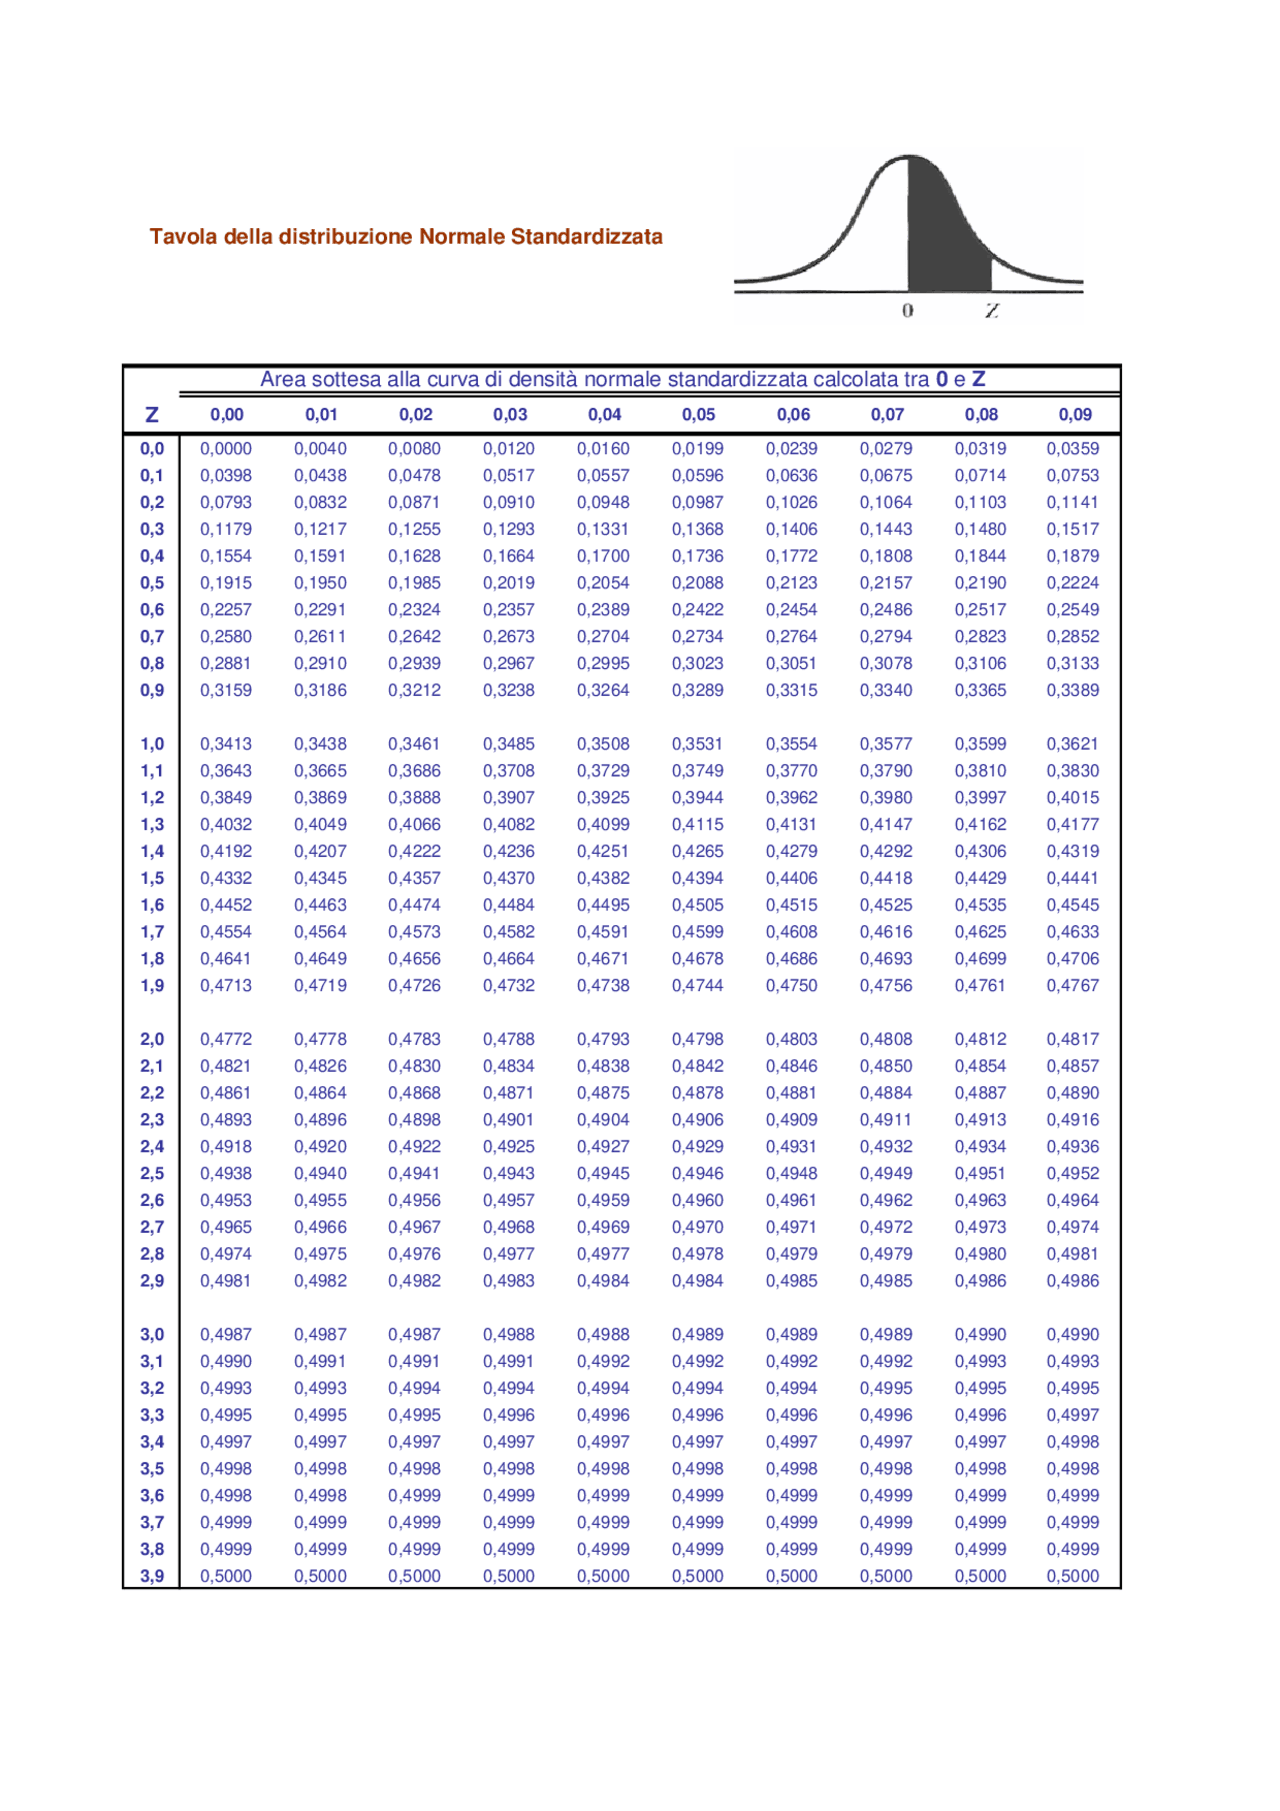
\includegraphics[width = .99\textwidth]{img/tab_gaus1}
    \end{minipage}
    \newpage
    \begin{minipage}{.99\textwidth}
        \centering
        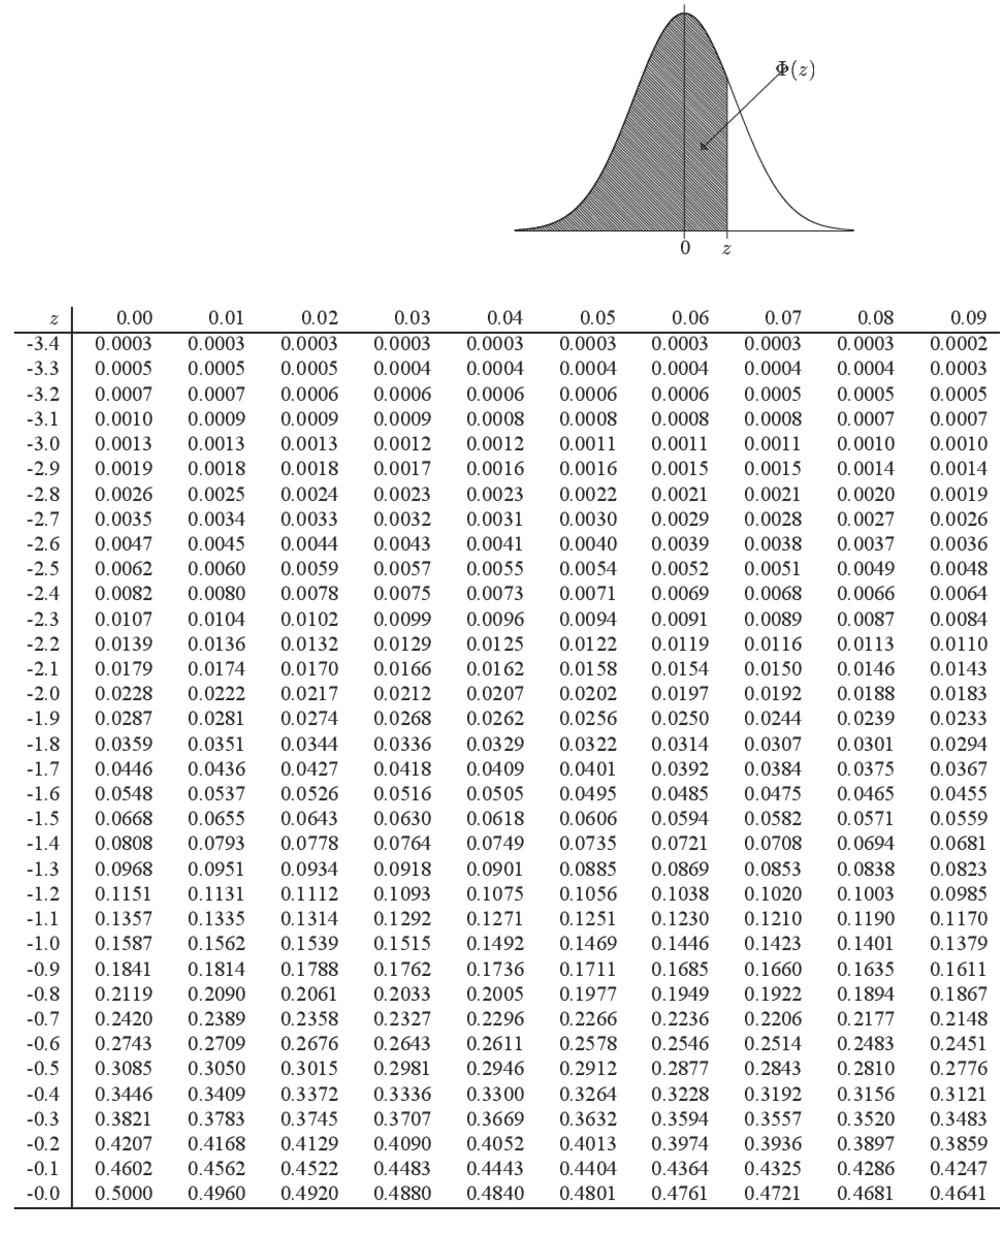
\includegraphics[width = .99\textwidth]{img/tab_gaus2}
    \end{minipage}


    \section{Student}

    \begin{minipage}{0.99\textwidth}
        \centering
        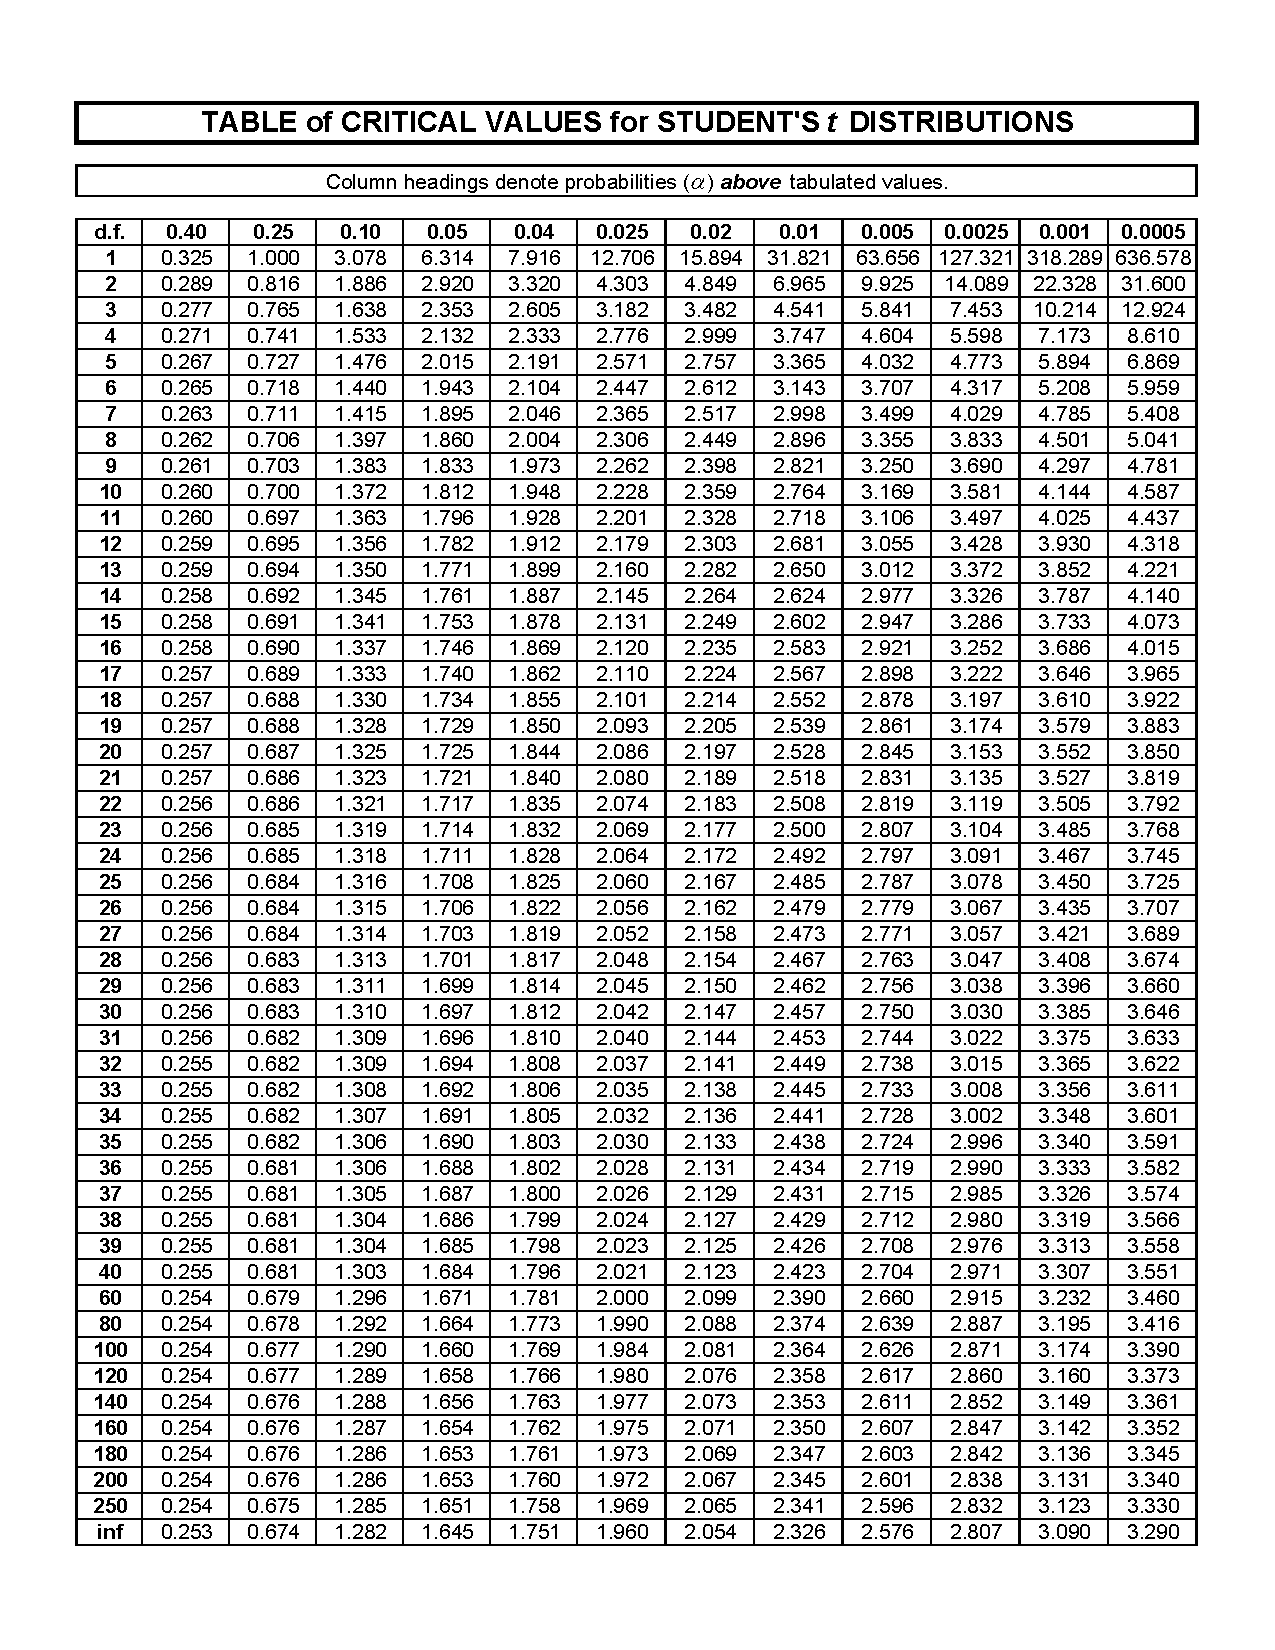
\includegraphics[width = .95\textwidth]{img/Tabella_Student}
    \end{minipage}

    \section{Correlazione lineare}
    \vspace*{\fill}
    \begin{minipage}{0.99\textwidth}
        \centering
        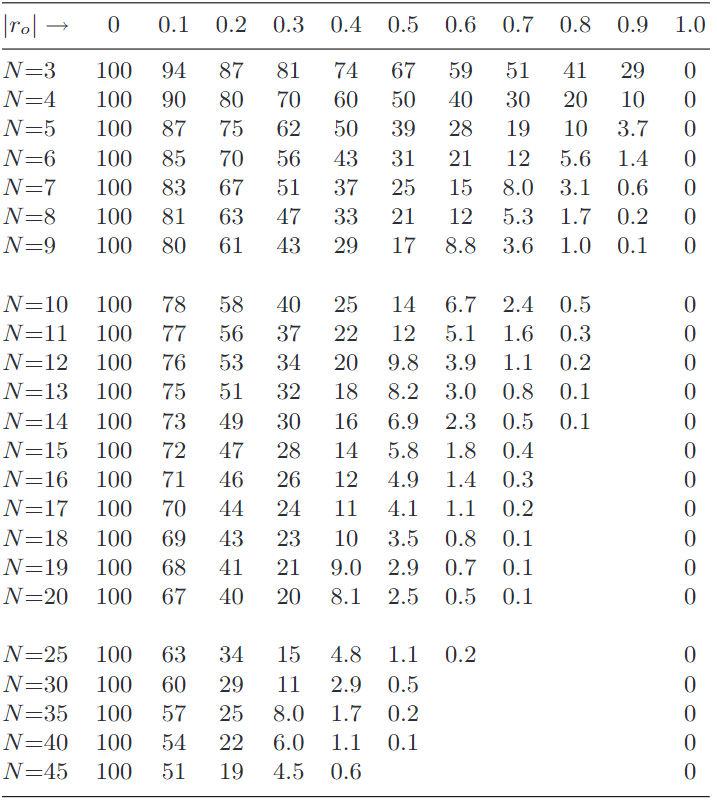
\includegraphics[width = .9\textwidth]{img/tab_r}
    \end{minipage}
    \vspace*{\fill}

    \section{$ \chi^2 $}
    \begin{minipage}{.99\textwidth}
        \centering
        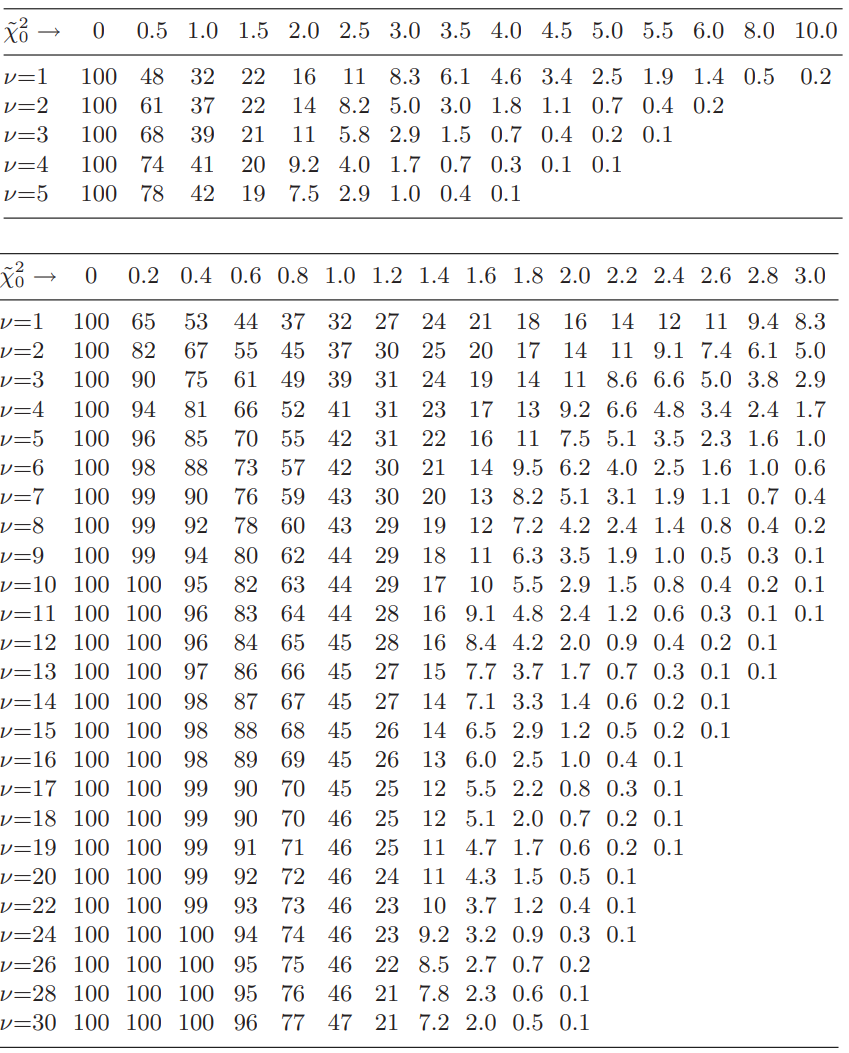
\includegraphics[width = .99\textwidth]{img/chi_table}
    \end{minipage}

    \bibliography{main}
    \bibliographystyle{plain}

\end{document}
